\chapter{الدورات البيوجيوكيميائية}\label{ch:b2:biogeochemical-cycles}

في آذار 1958 شغّل كيميائي شاب اسمه تشارلز كيلنغ
محللَ غازات بالأشعة تحت الحمراء على المنحدر الشمالي لمونا لوا، في هاواي،
على ثلاثة كيلومترات ونصف فوق المحيط الهادئ، حيث الهواء
ممتزج أحسن ما يكون امتزاج الهواء. وكان قد توقع قياس ثابت؛
وفي غضون سنة كان لديه سن منشار --- ثاني أكسيد الكربون يرتفع كل
شتاء ويهبط كل صيف إذ تزفر غابات نصف الكرة
الشمالي وتشهق --- وفي غضون بضع سنين ميل
تحت سن المنشار لم يتوقف منذئذ. \omterm{prop:b2:biogeochemical-cycles:carbon}{ومنحني كيلنغ}
هو تنفس المحيط الحيوي مرئيًا من الخارج، وعليه مرسوم مخطط
حمّى. وهذا الفصل في الدورات التي يسجلها المنحني:
أين يُخزن كربون الأحياء ونتروجينها وفوسفورها وكبريتها،
وكم بسرعة تنتقل بين \omterm{def:b2:biogeochemical-cycles:reservoir}{المستودعات}، وما الذي يقرر تلك
السرعات --- ومعظمها استقلابات
\cref{ch:b2:microbial-metabolism} --- وماذا فعل نوع واحد
بكل دورة في مئتي سنة.

\section{المستودعات والتدفقات وأزمنة المكث}

\begin{definition}[المستودع والتدفق وزمن المكث]\label{def:b2:biogeochemical-cycles:reservoir}
\index{مستودع}\index{تدفق}\index{زمن مكث}\index{حالة مستقرة}\index{دورة بيوجيوكيميائية}
\emph{الدورة البيوجيوكيميائية} انتقال عنصر بين
\emph{المستودعات} (الغلاف الجوي، والمحيط، والتربة، والكتلة الحيوية
الحية، والصخور) \emph{بتدفقات} تُقاس بالكتلة في السنة. والمستودع
الذي كتلته $M$ وخرجه الكلي $F$ له \emph{زمن
مكث} $\tau = M/F$، وهو الزمن الوسطي الذي تقضيه فيه ذرة؛ وعند
\emph{الحالة المستقرة} يساوي الداخل الخارج ويكون $M$ ثابتًا.
والدورات مقترنة بتكافؤ الحياة --- أي \emph{نسبة ردفيلد}
للعوالق البحرية، $\mathrm{C:N:P} =
106:16:1$ بالذرات --- بحيث يقرر توفر العنصر الأندر
المعدلَ الذي تُلتقط به سائر العناصر.
\end{definition}

\begin{theorem}[نموذج الصندوق الواحد]\label{thm:b2:biogeochemical-cycles:box}
\index{نموذج الصندوق}\index{زمن الاسترخاء}
إذا فقد \omterm{def:b2:biogeochemical-cycles:reservoir}{مستودع} محتواه بمعدل يتناسب مع ما
يحمله، $F_{\text{الخارج}} = M/\tau$، وتلقى دخلًا ثابتًا
$F_{\text{الداخل}}$، كان
\[
\frac{\mathrm{d}M}{\mathrm{d}t} = F_{\text{الداخل}} - \frac{M}{\tau},
\qquad
M(t) = M^{*} + (M_0 - M^{*})\,e^{-t/\tau}, \qquad M^{*} = F_{\text{الداخل}}\tau :
\]
فيسترخي \omterm{def:b2:biogeochemical-cycles:reservoir}{المستودع} إلى \omterm{def:b2:biogeochemical-cycles:reservoir}{حالة مستقرة} تتناسب مع دخله،
\omterm{def:b2:biogeochemical-cycles:reservoir}{وزمن المكث} ثابتُها الزمني. ورفع الدخل رفعةً واحدة
يرفع \omterm{def:b2:biogeochemical-cycles:reservoir}{الحالة المستقرة} بالتناسب ويتبعه \omterm{def:b2:biogeochemical-cycles:reservoir}{المستودع}
في غضون بضعة $\tau$: فالحوض الذي زمن مكثه أيام
(النشادر الجوي، ونترات بحيرة في الربيع) يتتبع
منابعه؛ والذي زمن مكثه قرون (كربون المحيط العميق،
والمادة العضوية في التربة) يكاملها، ويعمّر اضطراب الحوض
البطيء أطول من الاضطراب الذي سببه.
\end{theorem}
\begin{proof}
المعادلة خطية بمعاملات ثابتة: \omterm{def:b2:biogeochemical-cycles:reservoir}{فالحالة المستقرة}
$M^{*}$ تجعل الطرف الأيمن صفرًا، والانحراف $m = M - M^{*}$
يخضع للمعادلة $\dot m = -m/\tau$، فيكون $m = m_0 e^{-t/\tau}$. وإذا كان \omterm{def:b2:biogeochemical-cycles:reservoir}{للمستودع}
عدة مخارج، قرر مجموعها $\tau$، $1/\tau = \sum_i
1/\tau_i$: فيغلب أسرع المصارف.
\end{proof}

\section{دورة الكربون}

\begin{proposition}[ميزانية الكربون]\label{prop:b2:biogeochemical-cycles:carbon}
\index{دورة الكربون}\index{الكسر المحمول جوًا}\index{مصرف كربون}\index{منحني كيلنغ}
بوحدات الغيغاطن من الكربون (\unit{GtC}، أي $10^{12}$~kg)، تكون
\omterm{def:b2:biogeochemical-cycles:reservoir}{المستودعات} الرئيسة الغلاف الجوي (نحو 880 في عشرينيات هذا القرن، و590
قبل الصناعة)، ونباتات اليابسة (450)، والتربة (1700)، والمحيط
السطحي (900)، والمحيط العميق (\num{37000})، والصخور الرسوبية
(\num{e8})؛ والوقود الأحفوري هو الكسر من الأخيرة الذي
تستطيع الصناعة بلوغه، وهو نحو \num{5000}. والتدفقات الطبيعية كبيرة
وشبه متوازنة: فالتركيب الضوئي على اليابسة يأخذ نحو 120 في
السنة ويعيده التنفس والتحلل؛ ويتبادل سطح المحيط
نحو 80 في كل اتجاه مع الهواء. أما \omterm{def:b2:biogeochemical-cycles:reservoir}{التدفق} البشري
فصغير في مقابلها --- نحو 10 في السنة من الوقود الأحفوري و1
من إزالة الغابات --- لكنه أحادي الاتجاه، وقد أبقى الغلاف الجوي
\emph{نحو \qty{45}{\%}} منه (وهو \emph{\omterm{prop:b2:biogeochemical-cycles:carbon}{الكسر المحمول جوًا}})،
وأخذ المحيط ربعًا وأخذت اليابسة، وقد سمّدها
$\mathrm{CO_2}$ الزائد، الباقي. والجزء من المليون من $\mathrm{CO_2}$ الجوي هو
\qty{2.13}{GtC}؛ وارتفع التركيز من 280 إلى \num{315}~\unit{ppm}
بين 1750 و1958، ومن 315 إلى ما فوق \num{420} بين 1958
وعشرينيات هذا القرن، وهو يرتفع الآن بمقدار \qty{2.5}{ppm} في السنة. \omterm{def:b2:biogeochemical-cycles:reservoir}{وزمن
مكث} جزيء $\mathrm{CO_2}$ في الهواء، $880/200 \approx 4$ سنوات،
قصير؛ أما عمر \emph{الفائض}، وتقرره بطء
الامتزاج في المحيط العميق وتجوية الصخر الأبطأ، فهو
قرون إلى آلاف السنين --- فخُمس ما يُطلق اليوم سيظل
في الهواء بعد عشرة آلاف سنة.
\end{proposition}
\begin{proof}[شواهد]
ثلاثة توقيعات تبيّن أن الكربون المضاف أحفوري. أولها
نظائره: فالكربون الأحفوري لا $\mathrm{{}^{14}C}$ فيه (إذ تفكك
قبل ملايين السنين) وهو فقير في $\mathrm{{}^{13}C}$ كما هو كل كربون
نباتي، والغلاف الجوي ما زال يفقد الاثنين --- وهو أثر
سويس، المقيس في حلقات الأشجار منذ الخمسينيات. وثانيها أكسجينه:
أما $\mathrm{O_2}$ الغلاف الجوي فيهبط على الوتيرة نفسها، بتكافؤ
الاحتراق، كما بيّن ابن كيلنغ في التسعينيات، وهو ما لا ينتجه
منبع بركاني أو محيطي. وثالثها مسك الدفاتر: فمجموع
الفحم والنفط والغاز المباع، محوَّلًا إلى كربون، يفوق الزيادة
في الهواء بعامل اثنين، ويوجد النصف المفقود في
كربون المحيط اللاعضوي المنحل المرتفع وحموضته المتزايدة، وفي
مصرف اليابسة. وسن المنشار الموسمي، وهو أكبر في بارو في ألاسكا
منه في مونا لوا ويكاد يغيب عند القطب الجنوبي، هو التقاط الغابات
الشمالية في الصيف وإطلاقها في الشتاء --- أي قياس
مباشر لتنفس المحيط الحيوي.
\end{proof}

\begin{omfigure}
\begin{tikzpicture}
\begin{axis}[
  width=0.9\linewidth, height=6cm,
  axis x line=bottom, axis y line=left,
  xmin=1955, xmax=2026, ymin=300, ymax=430,
  xlabel={السنة}, ylabel={$\mathrm{CO_2}$ (\unit{ppm})، المتوسط السنوي في مونا لوا},
  xlabel style={font=\small, at={(axis description cs:0.5,-0.13)}, anchor=north},
  ylabel style={font=\small},
  tick label style={font=\small}, xtick={1960,1970,1980,1990,2000,2010,2020}, ytick={300,325,350,375,400,425},
  scaled x ticks=false, x tick label style={/pgf/number format/1000 sep=},
  clip=false,
]
\addplot[very thick, omDef, mark=*, mark size=1pt] coordinates {
(1959,316.0) (1962,318.5) (1965,320.0) (1968,323.0) (1971,326.3) (1974,330.2) (1977,333.8) (1980,338.8) (1983,342.8) (1986,347.2) (1989,353.1) (1992,356.4) (1995,360.8) (1998,366.7) (2001,371.1) (2004,377.5) (2007,383.8) (2010,389.9) (2013,396.5) (2016,404.2) (2019,411.4) (2022,418.5) (2024,424.6)};
\node[font=\scriptsize, anchor=north west, align=left] at (axis cs:1958,425) {الستينيات: \qty{+0.9}{ppm/yr}\\عشرينيات القرن الحادي والعشرين: \qty{+2.4}{ppm/yr}};
\node[font=\scriptsize, anchor=west, align=left] at (axis cs:1990,320) {المستوى قبل الصناعة: \qty{280}{ppm}؛\\وفي كل سنة يركب هذا الخط سن منشار قدره $\pm\qty{3}{ppm}$};
\end{axis}
\end{tikzpicture}

{\small \omterm{prop:b2:biogeochemical-cycles:carbon}{منحني كيلنغ}: المتوسط السنوي لثاني أكسيد الكربون في الهواء عند
مونا لوا منذ 1959. وقد كاد الميل يتثلث؛ وسن المنشار
الموسمي فوقه، وهو غير مبيّن بهذا المقياس، هو تركيب نصف
الكرة الشمالي الضوئي في الصيف.}
\end{omfigure}

\begin{omfigure}
\begin{tikzpicture}[every node/.style={font=\scriptsize}, >=stealth, box/.style={draw, rounded corners, minimum width=2.2cm, minimum height=0.9cm, align=center, fill=#1}]
  \node[box=omDef!15] (atm) at (0,3) {الغلاف الجوي\\880};
  \node[box=omThm!15] (veg) at (-4.4,0.6) {نباتات اليابسة 450\\التربة 1700};
  \node[box=omProp!15] (surf) at (4.4,0.6) {المحيط السطحي\\900};
  \node[box=omProp!25] (deep) at (4.4,-1.6) {المحيط العميق\\37\,000};
  \node[box=gray!20] (rock) at (0,-1.6) {الصخور والوقود الأحفوري\\$10^{8}$؛ والمتاح $\sim 5000$};
  \draw[->, thick] ([xshift=-2mm]atm.south west) -- node[above left, pos=0.45] {120 تركيب ضوئي} ([xshift=-4mm]veg.north);
  \draw[->, thick] ([xshift=5mm]veg.north) -- ([xshift=-2mm]atm.south); \node[anchor=north east] at (-0.4,1.5) {119 تنفس وحرائق};
  \draw[->, thick] ([xshift=2mm]atm.south east) -- node[above right, pos=0.45] {80 انحلال} ([xshift=4mm]surf.north);
  \draw[->, thick] ([xshift=-5mm]surf.north) -- ([xshift=2mm]atm.south); \node[anchor=north west] at (0.4,1.5) {78 تحرر غازي};
  \draw[<->, thick] (surf) -- node[right] {$\sim 100$ امتزاج وهبوط} (deep);
  \draw[->, very thick, omExo!80!black] (rock.north) -- node[left, align=right, pos=0.4] {10 وقود أحفوري\\ + 1 استعمال الأرض} (atm.south);
  \node[align=left, anchor=west] at (7.0,3.2) {التدفقات بوحدة \unit{GtC/yr}،\\ والمخزونات بوحدة \unit{GtC}\\[2pt] ومن 11 المنطلقة:\\ 5 تبقى في الهواء،\\ و3 إلى اليابسة،\\ و3 إلى المحيط};
\end{tikzpicture}

{\small \omterm{prop:b2:biogeochemical-cycles:carbon}{دورة الكربون} بأعداد مدوّرة. التبادلات الطبيعية
عشرة أمثال \omterm{def:b2:biogeochemical-cycles:reservoir}{التدفق} البشري، لكنها تكاد تتلاشى؛ أما \omterm{def:b2:biogeochemical-cycles:reservoir}{التدفق}
البشري فلا.}
\end{omfigure}

\begin{omfigure}
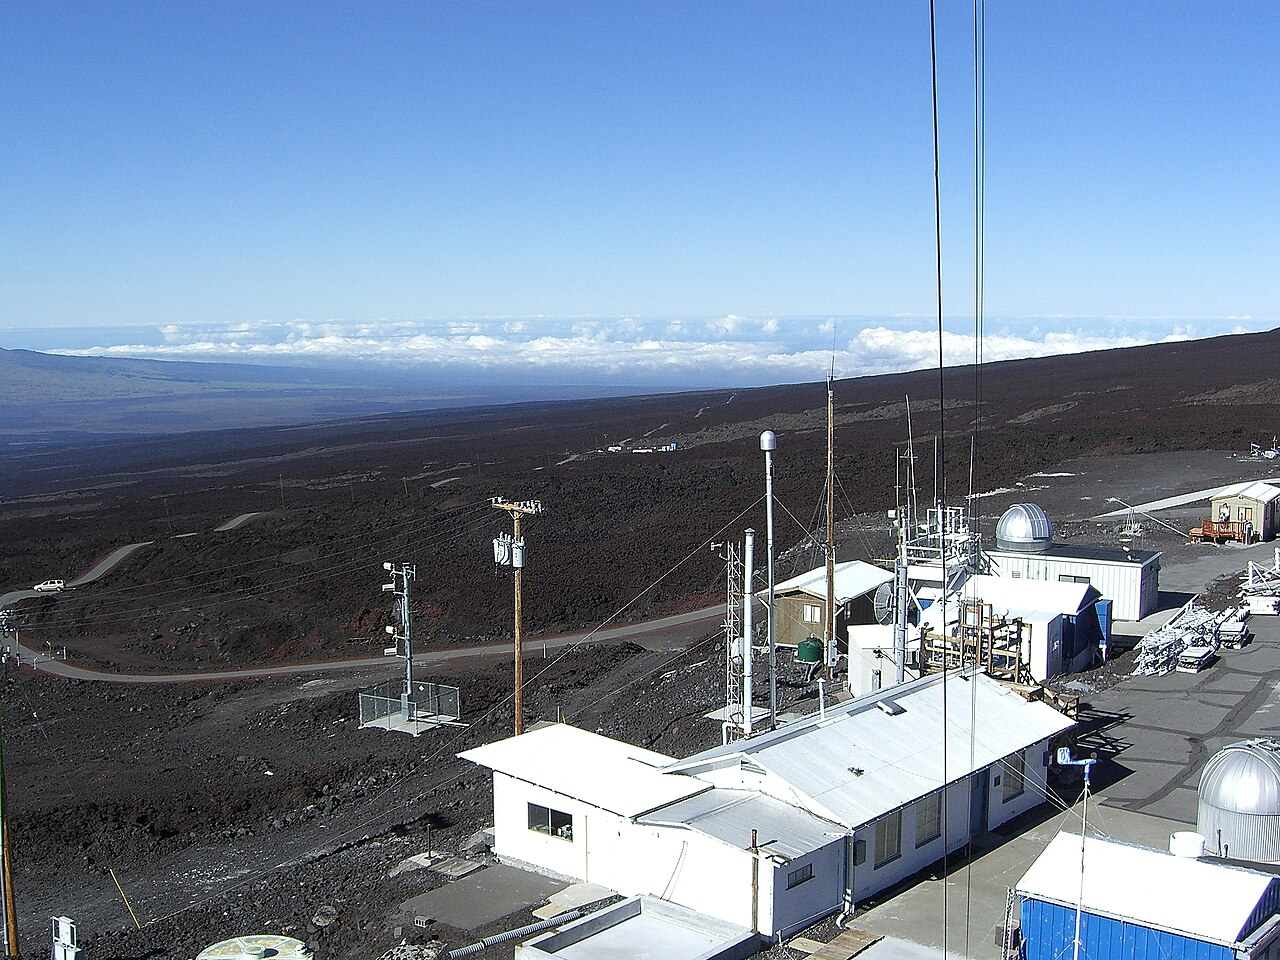
\includegraphics[width=0.56\linewidth]{images/book4/mauna-loa.jpg}\hspace{0.03\linewidth}
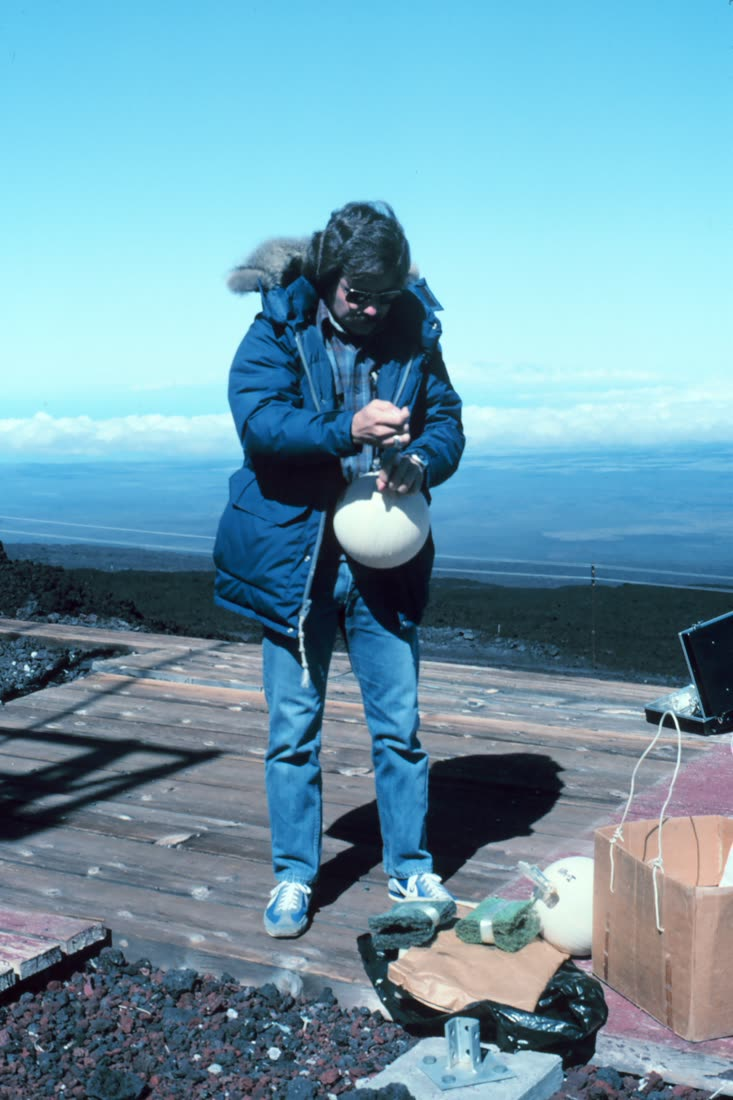
\includegraphics[width=0.33\linewidth]{images/book4/keeling-flask.jpg}

{\small حيث يُرسم المنحني. إلى اليسار: المرصد على
الجناح الشمالي لمونا لوا، على ارتفاع \qty{3400}{m}، فوق انقلاب
الرياح التجارية الذي يبقي هواء الجزيرة نفسها تحته. وإلى اليمين: أخذ عينة
بقارورة سنة 1982؛ وقوارير كهذه، تُحلَّل في
كاليفورنيا، تتحقق من المحلل المستمر وتُملأ في
محطات من ألاسكا إلى القطب الجنوبي.}
\end{omfigure}

\section{دورة النتروجين}

\begin{proposition}[دورة النتروجين]\label{prop:b2:biogeochemical-cycles:nitrogen}
\index{دورة النتروجين}\index{تثبيت النتروجين}\index{نترتة}\index{نزع النترتة}\index{طريقة هابر--بوش}\index{أناموكس}
النتروجين وافر --- فالهواء يحمل $4\times 10^{9}$~Tg من
$\mathrm{N_2}$ --- وشحيح، لأن الرابطة الثلاثية في $\mathrm{N_2}$ لا تفتحها
غير عمليتين: البرق (بضعة Tg في السنة)
\emph{والتثبيت الحيوي للنتروجين} ببدائيات النوى ذوات
النتروجيناز، وهو نحو 100 Tg في السنة على اليابسة و100 في البحر، بكلفة
16 ATP لكل $\mathrm{N_2}$. ثم يجري النتروجين المثبَّت في سلّم
إرجاع وأكسدة تسوقه المجهريات (\cref{ch:b2:microbial-metabolism}):
\emph{فالأمنجة} للمادة الميتة إلى $\mathrm{NH_4^{+}}$؛
و\emph{النترتة} من $\mathrm{NH_4^{+}}$ إلى $\mathrm{NO_2^{-}}$ و$\mathrm{NO_3^{-}}$ بذاتيات
التغذي الكيميائية الحجرية الهوائية؛ والتقاط $\mathrm{NH_4^{+}}$ أو $\mathrm{NO_3^{-}}$ بالنبات
وإرجاعه إلى أمين؛ وحيث يغيب الأكسجين،
\emph{\omterm{def:b2:microbial-metabolism:anaerobic}{نزع النترتة}} من $\mathrm{NO_3^{-}}$ إلى $\mathrm{N_2}$ (مع $\mathrm{N_2O}$
تسريبًا) و\emph{الأناموكس}، وهي أكسدة الأمونيوم اللاهوائية
بالنتريت إلى $\mathrm{N_2}$، وهما معًا يعيدان إلى الهواء نحو ما يأخذه
التثبيت. \omterm{def:b2:biogeochemical-cycles:reservoir}{وزمن مكث} ذرة نتروجين في
المحيط الحيوي بضع مئات من السنين؛ وفي الغلاف الجوي $4\times
10^{9}/400 \approx 10^{7}$ سنة. ومنذ 1913 ثبّتت طريقة \emph{هابر--بوش}
النتروجين صناعيًا، وهي الآن نحو 120 Tg في السنة،
وتضيف البقوليات المزروعة واحتراق الوقود الأحفوري 60 و30:
فالنشاط البشري يثبّت من النتروجين ما تثبّته العمليات الطبيعية
كلها معًا، ويطعم نصف الأحياء من الناس.
\end{proposition}

\begin{omfigure}
\begin{tikzpicture}[every node/.style={font=\scriptsize}, >=stealth, box/.style={draw, rounded corners, minimum width=1.9cm, minimum height=0.8cm, align=center, fill=#1}]
  \node[box=omDef!15] (n2) at (0,3.4) {$\mathrm{N_2}$ في الهواء\\$4\times 10^{9}$ Tg};
  \node[box=omThm!15] (org) at (-4.6,1.0) {نتروجين عضوي\\نبات وتربة وبحر};
  \node[box=omProp!15] (nh4) at (-2.2,-0.8) {$\mathrm{NH_4^{+}}$};
  \node[box=omProp!15] (no2) at (2.2,-0.8) {$\mathrm{NO_2^{-}}$};
  \node[box=omProp!15] (no3) at (4.6,1.0) {$\mathrm{NO_3^{-}}$};
  \draw[->, thick] (n2) -- node[above left, align=right] {تثبيت\\نتروجيناز، 200\\هابر--بوش 120} (org);
  \draw[->, thick] (org.south) -- node[below left] {أمنجة} (nh4.north);
  \draw[->, thick] (nh4) -- node[below] {نترتة} (no2);
  \draw[->, thick] (no2) -- node[below right] {نترتة} (no3);
  \draw[->, thick] (no3) to[bend left=18] node[above, pos=0.72] {استيعاب} (org);
  \draw[->, thick, omExo!80!black] (no3) -- node[above right, align=left] {نزع النترتة\\(لاأكسجيني)، وتسريب $\mathrm{N_2O}$} (n2);
  \draw[->, thick, omExo!80!black] (no2) -- node[right, pos=0.55, align=left] {أناموكس\\(مع $\mathrm{NH_4^{+}}$)} (n2);
  \node[anchor=north, align=center] at (0,-1.5) {التدفقات بوحدة Tg نتروجين في السنة؛ وكل خطوة عدا الاستيعاب والأمنجة تقوم بها بدائيات النوى};
\end{tikzpicture}

{\small \omterm{prop:b2:biogeochemical-cycles:nitrogen}{دورة النتروجين} سلّمًا للإرجاع والأكسدة (والنبات يستوعب
الأمونيوم كما يستوعب النترات). والتثبيت \omterm{def:b2:microbial-metabolism:anaerobic}{ونزع النترتة}، وهما
بابا الغلاف الجوي، مجهريان كلاهما؛ والباب الصناعي
صار يعادل الطبيعي.}
\end{omfigure}

\begin{proof}[شواهد]
غابة هَبَرد بروك التجريبية في نيوهامبشير: ففي 1965 قُطع
حوض تصريف كامل قطعًا جائرًا وأُبقي عاريًا بمبيد الأعشاب،
في حين تُرك حوض مجاور سليمًا، وقيست الجداول التي تصرّف
كلًّا منهما وحُلّلت سنين. ففقد الحوض المجرَّد
النتراتِ بستين ضعف معدل الشاهد --- إذ لم يعد النبات يلتقط
رأسمال التربة النتروجيني كله، فنُترِت وغُسل خارجًا،
حاملًا معه الكالسيوم والبوتاسيوم ومحمّضًا الجدول. وبيّنت
التجربة إحكام الدورة في غابة سليمة (فبضعة كيلوغرامات
من النتروجين تُفقد في الهكتار في السنة، في مقابل مئات تدور) وما الذي يكسره.
\end{proof}

\section{الفوسفور والكبريت}

\begin{proposition}[دورتان بلا غاز سريع]\label{prop:b2:biogeochemical-cycles:ps}
\index{دورة الفوسفور}\index{دورة الكبريت}\index{إتخام غذائي}\index{ثنائي مثيل الكبريتيد}
\emph{الفوسفور} لا صورة غازية له. وهو يدخل النظم البيئية
بتجوية الأباتيت في الصخر، وهي نحو 20 Tg في السنة على كل
سطح اليابسة، ويُعاد تدويره داخل التربة والبحيرات مرات كثيرة
--- فشاردة الفوسفات في ماء بحيرة سطحي تُلتقط في غضون
ساعات --- ويغادر إلى الرواسب، حيث يبقى
$10^{8}$ سنة، أي دورة صخرية. ولذلك كانت الحياة مقتصدة في الفوسفور
ومحدودة به: \omterm{def:b2:biogeochemical-cycles:reservoir}{فزمن المكث} في المحيط نحو
\num{20000} سنة، وفوسفات البحر العميق، إذ يرفعها الصعود
المائي، تقرر إنتاجيته. والتعدين ينقل اليوم من الفوسفور
إلى الأرض الزراعية نحو ما تطلقه التجوية، ويسبب جريانه إلى
البحيرات \emph{\omterm{prop:b2:biogeochemical-cycles:ps}{الإتخام الغذائي}}: أي ازدهار الطحالب، وتحللها،
واستهلاك الأكسجين، وموت السمك --- وقد بيّنت تجارب شندلر
على بحيرات كاملة في أونتاريو في السبعينيات، وفيها سُمّد نصف
بحيرة بالفوسفور دون النصف الآخر، أن الفوسفور
وحده هو الزناد، وأدت إلى إزالته من المنظفات.
أما \emph{الكبريت} فله دورة صخرية (الجبس والبيريت) وطور
غازي: $\mathrm{SO_2}$ البراكين والفحم، و$\mathrm{H_2S}$ الرواسب
اللاأكسجينية، و\emph{\omterm{prop:b2:biogeochemical-cycles:ps}{ثنائي مثيل الكبريتيد}} من العوالق البحرية، ونواتج
أكسدته تبذر الغيوم فوق المحيط. وقد ثلّث حرق الفحم
\omterm{def:b2:biogeochemical-cycles:reservoir}{تدفق} الكبريت إلى الهواء في القرن العشرين
وأعطى أوروبا وأمريكا الشمالية مطرهما الحمضي؛ ثم عكست المنقيات
ذلك في غضون عقود، إذ كان \omterm{def:b2:biogeochemical-cycles:reservoir}{زمن مكث} الدورة في الهواء
بضعة أيام.
\end{proposition}

\begin{omfigure}
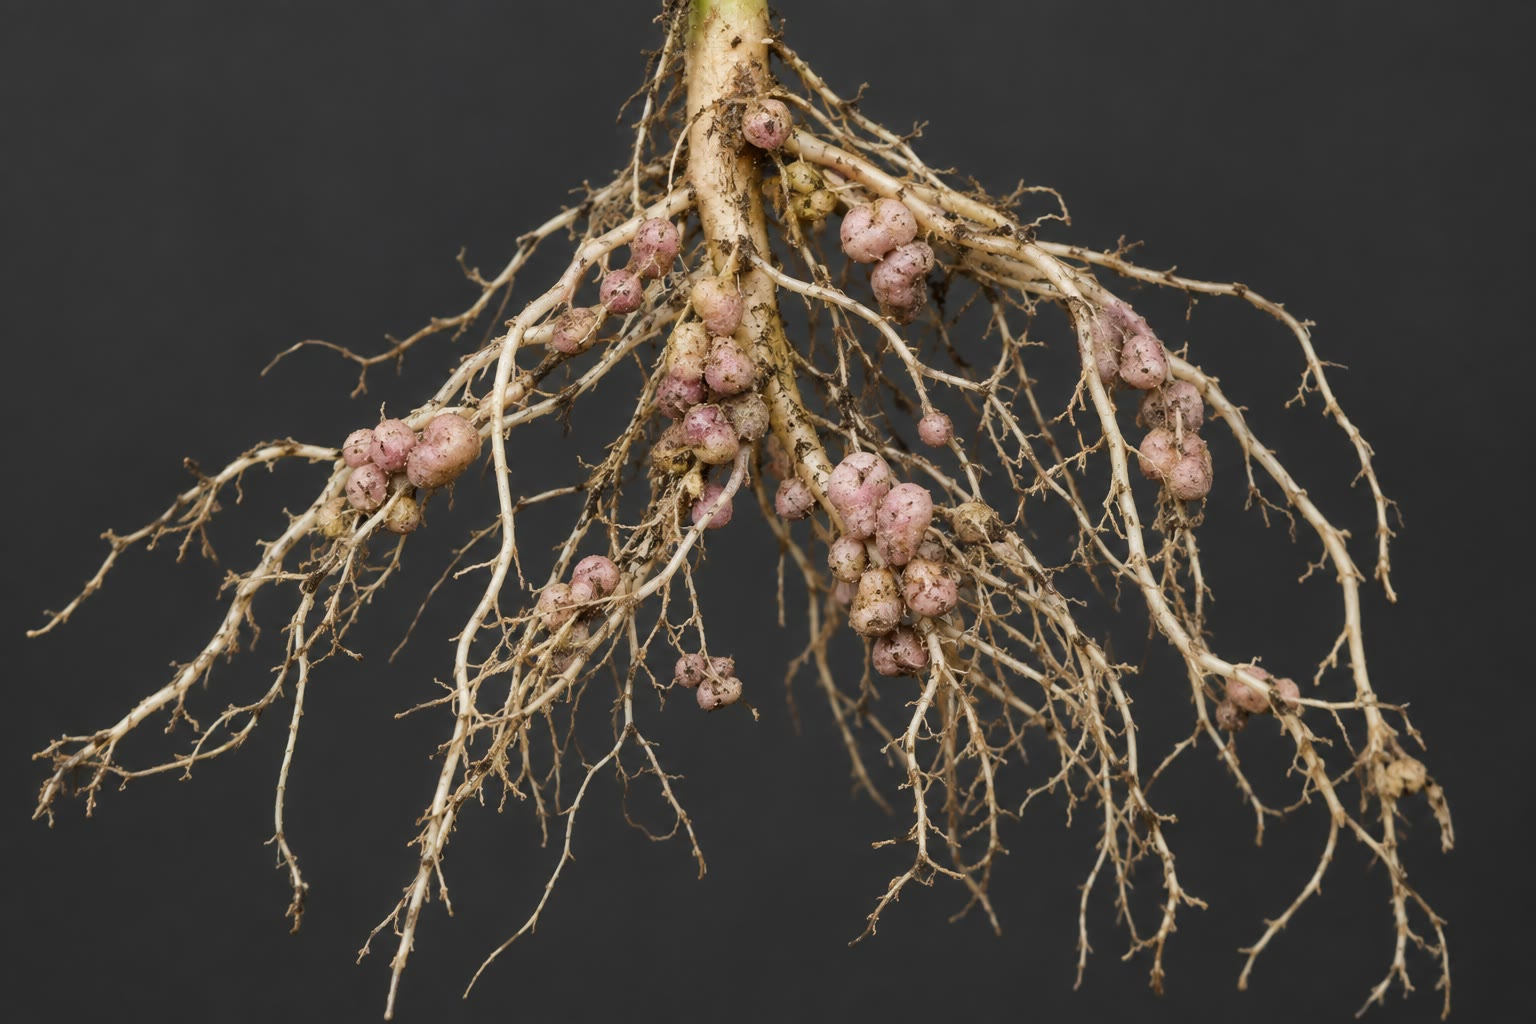
\includegraphics[width=0.44\linewidth]{images/book4/ai/b4-25-root-nodules.jpg}\hspace{0.04\linewidth}
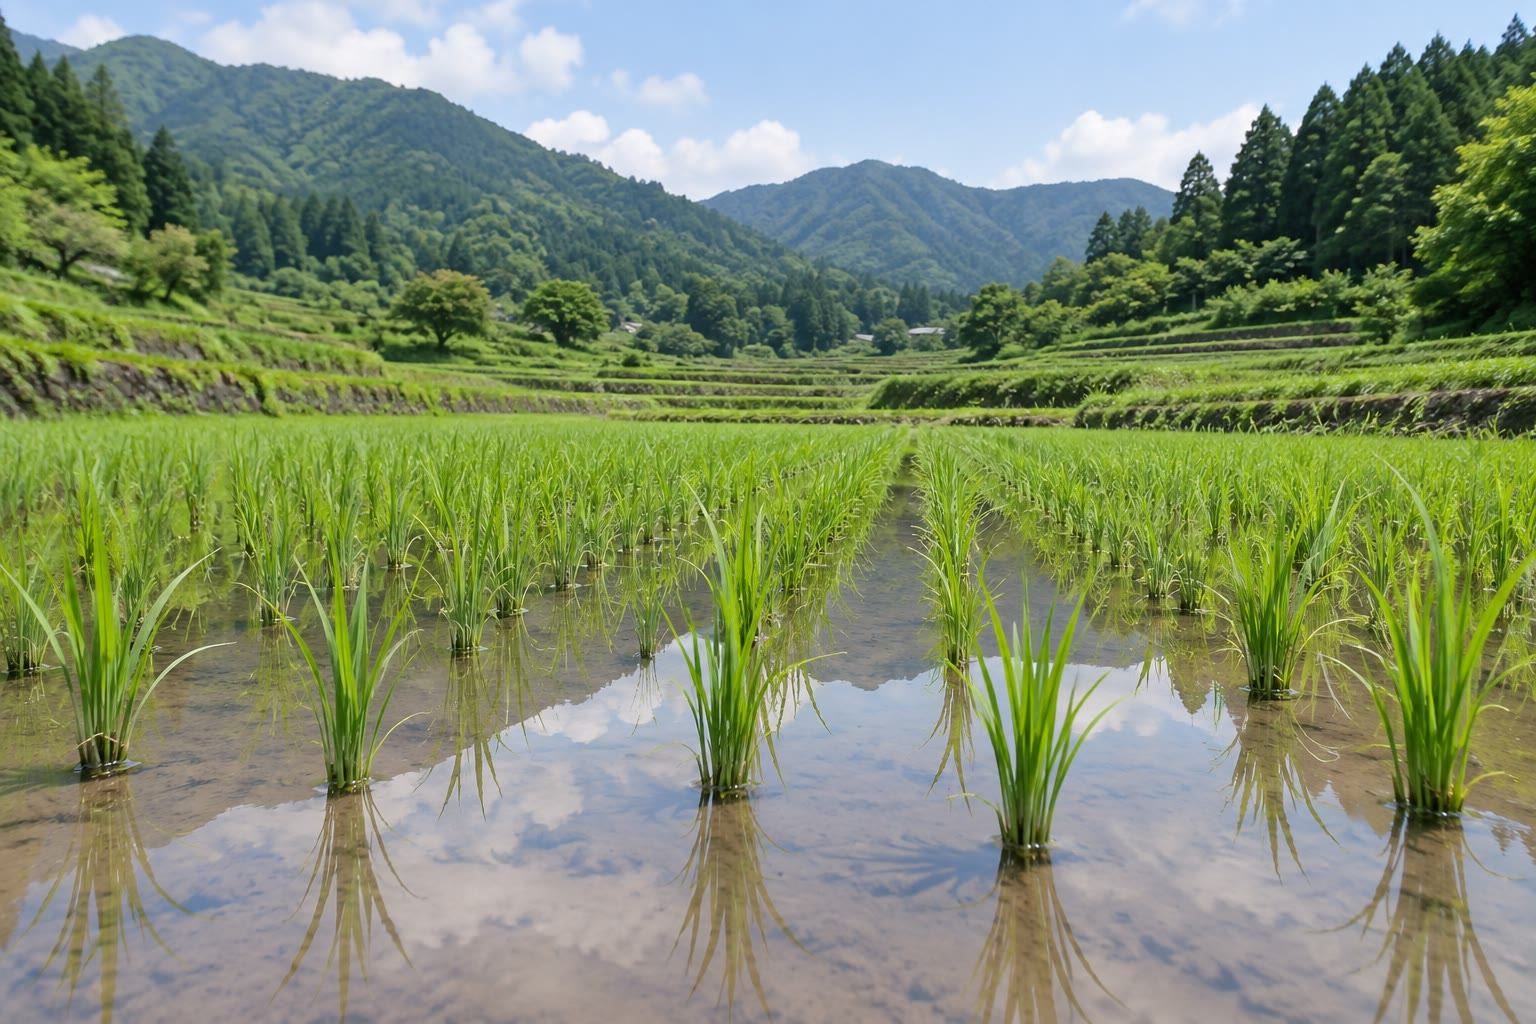
\includegraphics[width=0.44\linewidth]{images/book4/ai/b4-25-rice-paddy.jpg}

{\small بابا \omterm{prop:b2:biogeochemical-cycles:nitrogen}{دورة النتروجين}. إلى اليسار: عُقد جذرية عند
بقولية، كل منها حجرة تثبّت فيها الريزوبيا النتروجين لعائلها.
وإلى اليمين: حقل أرز مغمور، لاأكسجيني تحت السطح، حيث
يعيد \omterm{def:b2:microbial-metabolism:anaerobic}{نزع النترتة} النتروجين إلى الهواء وتصنع مولّدات الميثان
الميثان.}
\end{omfigure}

\section{الكوكب المضطرب}

\begin{example}[ما تقوله الأعداد]\label{ex:b2:biogeochemical-cycles:numbers}
انطلاقات قدرها \qty{10}{GtC} في السنة بكسر محمول جوًا قدره
$0.45$ تترك \qty{4.5}{GtC}، أي \qty{2.1}{ppm}، في الهواء كل سنة
--- وهو الميل الملحوظ. والانطلاقات المتراكمة منذ 1850 نحو
\qty{700}{GtC}، منها \qty{290}{GtC} في الهواء (140~\unit{ppm})، و
الباقي في المحيط واليابسة. ولإبقاء الغلاف الجوي عند أي مستوى، يجب
أن تهبط الانطلاقات الصافية إلى ما تستطيع المصارف البطيئة --- أي امتزاج المحيط العميق
والتجوية، وهما معًا دون \qty{1}{GtC} في السنة --- أخذه:
\emph{فالصفر الصافي} ليس شعارًا بل شرط \omterm{def:b2:biogeochemical-cycles:reservoir}{الحالة المستقرة}
في \omterm{thm:b2:biogeochemical-cycles:box}{نموذج الصندوق} عند $\tau$ طويل جدًا. وأما النتروجين، فمضاعفة
\omterm{def:b2:biogeochemical-cycles:reservoir}{تدفق} النتروجين المثبَّت ضاعفت النترات في الأنهار، وأنتجت
مناطق ميتة عند مصبي المسيسيبي والبلطيق، ورفعت
$\mathrm{N_2O}$ الغلاف الجوي، وهو غاز دفيئة زمن مكثه
قرن، بمقدار الخُمس. و\Cref{ch:b2:global-change} تتابع
العواقب على الأحياء.
\end{example}

\section{تمارين}

\begin{exercise}[$\star$]\label{exo:b2:biogeochemical-cycles:1}
عرّف \omterm{def:b2:biogeochemical-cycles:reservoir}{المستودع} \omterm{def:b2:biogeochemical-cycles:reservoir}{والتدفق} \omterm{def:b2:biogeochemical-cycles:reservoir}{وزمن المكث}، واحسب
\omterm{def:b2:biogeochemical-cycles:reservoir}{زمن مكث} الكربون في نباتات اليابسة (450 GtC، والتركيب الضوئي
120 GtC في السنة) وفي المحيط العميق (\num{37000} GtC، والتبادل
نحو 100 GtC في السنة).
\end{exercise}

\begin{exercise}[$\star$]\label{exo:b2:biogeochemical-cycles:2}
حوّل \qty{2.5}{ppm} في السنة إلى GtC، وحوّل \qty{10}{GtC} من
الانطلاقات إلى \unit{ppm}.
\end{exercise}

\begin{exercise}[$\star$]\label{exo:b2:biogeochemical-cycles:3}
سمِّ العمليتين الطبيعيتين اللتين تفتحان $\mathrm{N_2}$، والعملية التي
تعيده، وخطوات الإرجاع والأكسدة الثلاث بينهما، مع
الكائنات المسؤولة.
\end{exercise}

\begin{exercise}[$\star$]\label{exo:b2:biogeochemical-cycles:4}
لماذا يحد الفوسفور الإنتاجية أكثر من النتروجين
على المدى الجيولوجي، ويحدها النتروجين أكثر من الفوسفور في
موسم معطى؟
\end{exercise}

\begin{exercise}[$\star\star$]\label{exo:b2:biogeochemical-cycles:5}
بحيرة حجمها \qty{e7}{m^3} تتلقى \qty{2}{t} من الفوسفور في السنة
وتغسل \qty{20}{\%} من مائها سنويًا. احسب تركيز الفوسفور
في حالتها المستقرة والزمن اللازم لبلوغ \qty{90}{\%}
منه بعد بدء الدخل. وماذا لو نُصّف الدخل؟
\end{exercise}

\begin{exercise}[$\star\star$]\label{exo:b2:biogeochemical-cycles:6}
من معطيات كيلنغ، احسب معدل نمو $\mathrm{CO_2}$ الوسطي في
الستينيات (من 316 إلى \qty{325}{ppm} على مدى عشر سنين) وفي العقد الثاني من هذا القرن
(من 390 إلى 411 على مدى تسع سنين)، بوحدة \unit{ppm} في السنة وبوحدة \unit{GtC} في السنة.
\end{exercise}

\begin{exercise}[$\star\star$]\label{exo:b2:biogeochemical-cycles:7}
سعة سن المنشار الموسمي في مونا لوا نحو
\qty{6}{ppm} من الذروة إلى القاع. حوّلها إلى GtC وقارنها
بالإنتاج الأولي الصافي السنوي ليابسة نصف الكرة الشمالي،
وهو نحو \qty{35}{GtC}. ولماذا كان سن المنشار أصغر بكثير؟
\end{exercise}

\begin{exercise}[$\star\star$]\label{exo:b2:biogeochemical-cycles:8}
ينفق النتروجيناز 16 ATP لكل $\mathrm{N_2}$. ولبقولية تثبّت
\qty{200}{kg} من النتروجين في الهكتار في السنة، احسب مولات
$\mathrm{N_2}$ المثبَّتة وATP المنفق، وكتلة الغلوكوز التي يمثلها ذلك
ATP (نحو 30 ATP لكل غلوكوز). وأي كسر من ناتج التركيب الضوئي
لمحصول قدره \qty{10}{t/ha} يكون ذلك؟
\end{exercise}

\begin{exercise}[$\star\star$]\label{exo:b2:biogeochemical-cycles:9}
تنمو العوالق عند نسبة ردفيلد $\mathrm{C:N:P} = 106:16:1$.
وماء البحر في العمق يحمل \qty{2.2}{\micro mol/kg} من الفوسفات
و\qty{32}{\micro mol/kg} من النترات. فأيهما ينفد أولًا حين تُرفع
كتلة ماء إلى السطح، وكم كربونًا يُثبَّت قبل أن
ينفد؟
\end{exercise}

\begin{exercise}[$\star\star\star$]\label{exo:b2:biogeochemical-cycles:10}
عامل الغلاف الجوي صندوقًا فيه كربون فائض $E$ يُزال بمعدل
$E/\tau$ بالمصارف ويُغذى بانطلاقات $Q$. فعند $\tau =
50$ سنة و$Q = \qty{10}{GtC/yr}$، ما الفائض في \omterm{def:b2:biogeochemical-cycles:reservoir}{الحالة المستقرة}
وأي \unit{ppm} يوافقه؟ وفسّر لماذا يكون الجواب الحقيقي أسوأ.
\end{exercise}

\begin{exercise}[$\star\star\star$]\label{exo:b2:biogeochemical-cycles:11}
ضاعفت تجارب القنابل $\mathrm{{}^{14}C}$ الغلاف الجوي سنة 1963؛ ثم هبط
الفائض إلى النصف كل 11 سنة أو نحوها، مع أن $\mathrm{{}^{14}C}$
عمر نصفه 5730 سنة. فسّر ما الذي قيس، وبماذا
تخبرك السنوات 11 عن \omterm{prop:b2:biogeochemical-cycles:carbon}{دورة الكربون}.
\end{exercise}

\begin{exercise}[$\star\star\star$]\label{exo:b2:biogeochemical-cycles:12}
«ضاعف البشر \omterm{prop:b2:biogeochemical-cycles:nitrogen}{دورة النتروجين} ولم يفعلوا \omterm{prop:b2:biogeochemical-cycles:carbon}{بدورة الكربون} غير
الوكز.» ناقش بالأعداد: التدفقات المثبَّتة، وكسورها من
\omterm{def:b2:biogeochemical-cycles:reservoir}{التدفق} الطبيعي، \omterm{def:b2:biogeochemical-cycles:reservoir}{والمستودعات} المتأثرة.
\end{exercise}

\section{مسألة: ميزانية كربون قرن}

\begin{problem}[{مسألة نهاية الأسبوع --- قرن من الانطلاقات
مُمَرَّر عبر نموذج صندوق الغلاف الجوي، وحصة المحيط
وحصة اليابسة، وشلال النتروجين من حقل مسمَّد إلى
منطقة ميتة، وميزانية فوسفور بحيرة، وتنتهي إلى الكسر
المحمول جوًا، والتركيز الجوي سنة 2100، والنتروجين
المفقود في الهكتار}]
\label{pb:b2:biogeochemical-cycles:1}
المعطيات. الغلاف الجوي سنة 1850: \qty{285}{ppm}؛ و\qty{1}{ppm} $=
\qty{2.13}{GtC}$. والانطلاقات المتراكمة 1850--2020: \qty{700}{GtC}؛
و$\mathrm{CO_2}$ الجوي سنة 2020: \qty{412}{ppm}. وحقل مساحته
\qty{1}{ha} يتلقى \qty{150}{kg} من سماد النتروجين في السنة؛
ويلتقط المحصول \qty{60}{\%}، وتُنزع نترتة \qty{25}{\%}، ويُغسل
الباقي. وبحيرة حجمها \qty{5e7}{m^3} تغسل عُشر مائها
في السنة وتتلقى \qty{5}{t} من الفوسفور في السنة.

\medskip
\noindent\textbf{الجزء الأول --- \omterm{prop:b2:biogeochemical-cycles:carbon}{الكسر المحمول جوًا}.}
\begin{enumerate}
  \item احسب الكربون الجوي سنة 1850 وسنة 2020، و
        الزيادة بوحدة \unit{GtC}.
  \item احسب \omterm{prop:b2:biogeochemical-cycles:carbon}{الكسر المحمول جوًا} على مدى 1850--2020.
  \item وأين الباقي؟ أعطِ المصرفين، وأعطِ من
        القضية حصتيهما التقريبيتين.
  \item إذا كان المحيط قد أخذ \qty{25}{\%} من الانطلاقات، فبكم
        ارتفع كربونه اللاعضوي المنحل، \qty{38000}{GtC},
        نسبيًا؟ ولماذا يتحمض المحيط السطحي مع ذلك
        تحمضًا قابلًا للقياس؟
  \item لماذا يبقى \omterm{prop:b2:biogeochemical-cycles:carbon}{الكسر المحمول جوًا} ثابتًا تقريبًا في حين
        تنمو الانطلاقات نموًا أسّيًا؟ (افحص \omterm{thm:b2:biogeochemical-cycles:box}{نموذج الصندوق} عند
        $Q \propto e^{t/T}$ ومصرف $E/\tau$.)
  \item ماذا كان سيصير \omterm{prop:b2:biogeochemical-cycles:carbon}{الكسر المحمول جوًا} لو أُبقيت
        الانطلاقات ثابتة قرونًا كثيرة؟
\end{enumerate}

\medskip
\noindent\textbf{الجزء الثاني --- القرن القادم.}
نمذج الكربون الفائض $E$ (فوق مستوى 1850) بالمعادلة
$\mathrm{d}E/\mathrm{d}t = Q - E/\tau$، عند $\tau = 100$ سنة.
\begin{enumerate}[resume]
  \item احسب الفائض سنة 2020 بوحدة \unit{GtC}.
  \item مع إبقاء $Q$ عند \qty{10}{GtC/yr}، احسب الفائض في \omterm{def:b2:biogeochemical-cycles:reservoir}{الحالة
        المستقرة} والتركيز الذي يقتضيه.
  \item حُلّ لأجل $E(t)$ من 2020 عند $Q = 10$ وأعطِ $E$ سنة
        2100 والتركيز.
  \item ثم دع $Q$ يهبط خطيًا إلى الصفر بين 2020 و2070 و
        يبقى عند الصفر. احسب $E$ سنة 2070 (بمكاملة المعادلة؛
        فالحل الخاص لأجل $Q$ خطي هو خطي زائد
        ثابت) وسنة 2100.
  \item قارن التركيزين سنة 2100.
  \item لماذا كان $\tau$ واحد متفائلًا في السيناريو الثاني؟
\end{enumerate}

\medskip
\noindent\textbf{الجزء الثالث --- شلال النتروجين.}
\begin{enumerate}[resume]
  \item احسب النتروجين الذي يلتقطه المحصول والذي تُنزع نترتته والذي
        يُغسل، في الهكتار في السنة.
  \item يبلغ النتروجين المغسول نهرًا نتراتٍ ثم يبلغ
        البحر، حيث تستعمله العوالق بنسبة ردفيلد. فكم
        كربونًا يتيح للعوالق أن تثبّت؟
  \item ذلك الكربون يهبط ويُتنفَّس في العمق، فيستهلك
        الأكسجين بمعدل $\mathrm{O_2}$ واحد لكل C. احسب الأكسجين المستهلك، بالمول
        وبالكيلوغرام.
  \item المتر المكعب من ماء البحر يحمل نحو \qty{0.25}{mol} من
        $\mathrm{O_2}$ حين يكون مشبعًا. فكم مترًا مكعبًا من الماء القاعي
        ينزع غسلُ هكتار واحد أكسجينَه؟
  \item يفلت الكسر المنزوعة نترتته جزئيًا بصيغة $\mathrm{N_2O}$، وهو
        \qty{1}{\%} من النتروجين المنزوعة نترتته. احسب $\mathrm{N_2O}$
        في الهكتار في السنة، ومكافئه التدفئي بدلالة $\mathrm{CO_2}$
        (إذ يعادل $\mathrm{N_2O}$ 270 مرة $\mathrm{CO_2}$ في الكيلوغرام).
  \item قارن ذلك بما ينطلق من $\mathrm{CO_2}$ في صنع السماد
        (نحو \qty{4}{kg} من $\mathrm{CO_2}$ لكل كيلوغرام نتروجين
        \omterm{prop:b2:biogeochemical-cycles:nitrogen}{بطريقة هابر--بوش}).
\end{enumerate}

\medskip
\noindent\textbf{الجزء الرابع --- البحيرة.}
\begin{enumerate}[resume]
  \item احسب \omterm{def:b2:biogeochemical-cycles:reservoir}{زمن مكث} الفوسفور في البحيرة إذا كان الفقد
        الوحيد هو الغسل، وتركيزه في \omterm{def:b2:biogeochemical-cycles:reservoir}{الحالة المستقرة} بوحدة
        \unit{mg/m^3}.
  \item البحيرات التي فيها أكثر من \qty{30}{mg/m^3} من الفوسفور
        متخمة. فهل هذه منها؟
  \item يزيل الترسيب الفوسفور بثابت زمني خاص به
        قدره 5 سنوات. أعد حساب \omterm{def:b2:biogeochemical-cycles:reservoir}{زمن المكث} و
        التركيز.
  \item يُخفض الدخل إلى \qty{1}{t} في السنة. احسب \omterm{def:b2:biogeochemical-cycles:reservoir}{الحالة المستقرة}
        الجديدة والزمن اللازم للاقتراب منها إلى حدود \qty{10}{\%}.
  \item لماذا تتعافى بحيرات كثيرة أبطأ مما يتنبأ به هذا
        الحساب؟
  \item احسب الكربون الذي يستطيع فوسفور البحيرة بناءه في
        العوالق كل سنة بنسبة ردفيلد، من الدخل البالغ
        \qty{5}{t}.
  \item اذكر النتيجة: \omterm{prop:b2:biogeochemical-cycles:carbon}{الكسر المحمول جوًا}، والتركيزين
        سنة 2100، والنتروجين المغسول في
        الهكتار.
\end{enumerate}
\end{problem}
